% Source printed pp. 214-225 / PDF pp. 222-233.
\section{结点曲线}\label{src:6.2}
\begin{epigraph}
对我来说, [做]数学就像一次漫长的徒步旅行, 没有现成的路径, 也望不到终点.
\epigraphauthor{Maryam Mirzakhani}
\end{epigraph}
给出结点的刻画 (\bookref{6.2.4}) 后, 我们讨论亏格公式 (\bookref{6.2.12}), 对偶化层 (定义~\bookref{6.2.18}) 及结点曲线族的局部结构 (\bookref{6.2.26}).
\subsection{结点}\label{src:6.2.1-subsection}
\begin{definition}[结点]\label{src:6.2.1}
设 $C$ 是域 $k$ 上的曲线.
\begin{itemize}
\item 若存在同构 $\widehat{\mathcal O}_{C,\allowbreak p}\cong k[[x,\allowbreak y]]/(xy)$, 则称 $p\in C(k)$ 是\newterm{分裂结点}{split node}.
\item 若存在 $p$ 上方的分裂结点 $\overline p\in C_{\overline k}$, 则称闭点 $p\in C$ 是\textit{结点}.
\end{itemize}
若曲线 $C$ 纯一维, 且每个闭点均为光滑点或结点, 则称 $C$ 是\textit{结点曲线} (或\textit{至多具有结点奇点}).
\end{definition}
\begin{figure}[H]
\centering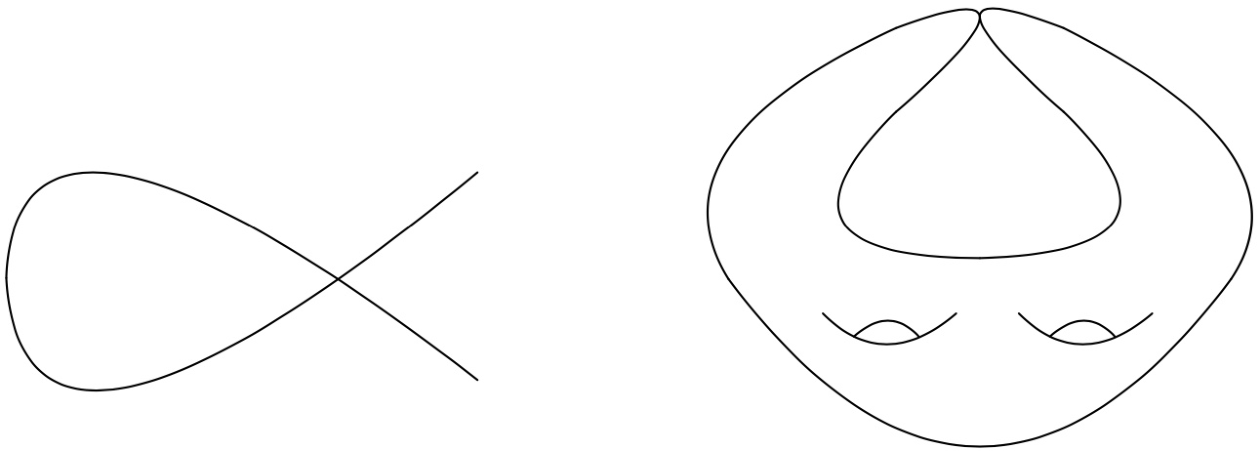
\includegraphics[width=.55\textwidth]{figures/fig-6.2.2.png}
\caption{$\mathbb C$ 上曲线的结点的代数视图 (左) 和解析视图 (右).}\label{src:6.2.2}
\end{figure}
\begin{example}\label{src:6.2.3}
\begin{enumerate}[(1)]
\item 曲线 $C=\Spec k[x,\allowbreak y]/(xy)$ 在 $0$ 处有分裂结点. 正规化 $\widetilde C\cong\mathbb A^1\coprod\mathbb A^1$ 的坐标环是 $k[x]\times k[y]$, 且 $\Gamma(C,\allowbreak \mathcal O_C)=\{(f,\allowbreak g)\in\Gamma(\widetilde C,\allowbreak \mathcal O_{\widetilde C})\mid f(0)=g(0)\}$. 换言之, $C$ 是 Ferrand 推出 (\bookref{B.4.1})
\[
\begin{tikzcd}
\Spec k\coprod\Spec k\arrow[r,"0\coprod0"]\arrow[d]&\widetilde C\arrow[d]\\
\Spec k\arrow[r,"0"']\arrow[ur,phantom,"\lrcorner",very near start]&C.
\end{tikzcd}
\]
\item 结点三次曲线 $C=\Spec k[x,\allowbreak y]/(y^2-x^2(x+1))$ 在 $0$ 处有分裂结点. 正规化 $\widetilde C\cong\mathbb A^1$ 具有坐标 $t=y/x$, 且 $x=t^2-1$, $y=t^3-t$; $C$ 同样是将 $\widetilde C$ 中 $0$ 的两个原像粘合所得的 Ferrand 推出.
\item 曲线 $C=\Spec\mathbb R[x,\allowbreak y]/(x^2+y^2)$ 在 $0$ 处有结点, 但它不是分裂结点, 因为二次型 $x^2+y^2$ 不分裂为线性因子.
\item 曲线 $\Spec\mathbb Q[x,\allowbreak y]/((x^2-2)(y^2-3))$ 在极大理想 $(x^2-2,\allowbreak y^2-3)$ 定义的点 $p$ 处有非分裂结点. 与前面结点为有理点的例子不同, $p$ 不是有理点, 域扩张 $\mathbb Q\to\kappa(p)$ 的次数为 $4$.
\item 设 $k\to\allowbreak k'$ 是次数为 $2$ 的可分域扩张, $C$ 是 $k$-代数 $\{f\in k'[x]\mid f(0)\in k\}$ 定义的 $k$ 上仿射曲线. 换言之, $C$ 是原点的包含 $0:\Spec k'\hookrightarrow\mathbb A_{k'}^1$ 沿 $\Spec k'\to\Spec k$ 的 Ferrand 推出. 曲线 $C$ 在一个 $k$-有理点处有非分裂结点.
\end{enumerate}
\end{example}
\subsection{结点的等价刻画}\label{src:6.2.2-subsection}
回顾 \S\bookref{A.3.4-subsection}, 曲线 $C$ 的奇异轨迹 $\operatorname{Sing}(C)$ 在概形意义下定义为 $\Omega_C$ 的第一个 Fitting 理想层的零点概形: 局部地, 若 $C=V(f_1,\allowbreak \ldots,\allowbreak f_m)\subseteq\mathbb A^n$, 则 $\operatorname{Sing}(C)$ 由 Jacobian 矩阵 $J=(\frac{\partial f_i}{\partial x_i})$ 的所有 $(n-1)\times(n-1)$ 子式的零点定义; 注意若 $C=V(f)\subseteq\mathbb A^2$ 是平面仿射曲线, 则 $\operatorname{Sing}(C)=V(\frac{\partial f}{\partial x},\allowbreak \frac{\partial f}{\partial y})$. 我们还将使用 \S\bookref{A.3.5-subsection} 讨论的局部完全交的性质.
\begin{proposition}[结点的刻画]\label{src:6.2.4}
设 $C$ 是域 $k$ 上的纯一维曲线, $p\in C$ 是闭点, 具有极大理想 $\mathfrak m\subseteq\mathcal O_{C,\allowbreak p}$. 以下条件等价:
\begin{enumerate}[(1)]
\item $p\in C$ 是结点;
\item $C$ 在 $p$ 处是局部完全交, 且 $\operatorname{Sing}(C)$ 在 $p\in\operatorname{Sing}(C)$ 处在 $k$ 上非分歧;
\item $k\to\kappa(p)$ 可分, $\mathcal O_{C,\allowbreak p}$ 约化, $\dim\mathfrak m/\mathfrak m^2=2$, 且存在映到 $\mathfrak m^2/\mathfrak m^3$ 中的 $0$ 的非退化二次型 $q\in\operatorname{Sym}^2\mathfrak m/\mathfrak m^2$;
\item $k\to\kappa(p)$ 可分且 $\widehat{\mathcal O}_{C,\allowbreak p}\cong\kappa(p)[[x,\allowbreak y]]/(q)$, 其中 $q$ 是非退化二次型; 且
\item 存在有限可分域扩张 $k\to\allowbreak k'$ 和点 $p'\in C_{k'}$, 使得 $\widehat{\mathcal O}_{C_{k'},\allowbreak p'}\cong k'[[x,\allowbreak y]]/(xy)$.
\end{enumerate}
\end{proposition}
\begin{proof}
假设 (1), 设 $\overline p\in C_{\overline k}$ 是 $p$ 上方的结点, $\operatorname{Sing}(C)\subseteq C$ 是概形意义的奇异轨迹. 由 Fitting 理想的性质 (见 \S\bookref{A.3.4-subsection}), $\operatorname{Sing}(C)\times_k\overline k=\operatorname{Sing}(C_{\overline k})$, 且 $\operatorname{Sing}(C_{\overline k})$ 在 $\Spec\widehat{\mathcal O}_{C_{\overline k},\allowbreak \overline p}\to\allowbreak C_{\overline k}$ 下的原像是 $\operatorname{Sing}(\Spec\widehat{\mathcal O}_{C_{\overline k},\allowbreak \overline p})$. 由于 $\widehat{\mathcal O}_{C_{\overline k},\allowbreak \overline p}\cong\overline k[[x,\allowbreak y]]/(xy)$, 有 $\operatorname{Sing}(\Spec\widehat{\mathcal O}_{C_{\overline k},\allowbreak \overline p})=V(x,\allowbreak y)=\Spec\overline k$. 因此 $\operatorname{Sing}(C)\to\Spec k$ 在 $p$ 处非分歧. 由于 $\widehat{\mathcal O}_{C_{\overline k},\allowbreak \overline p}$ 是完全交, $C$ 在 $p$ 处是局部完全交 (命题~\bookref{A.3.16}). 这得到 (2).

假设 (2), 由于 $\operatorname{Sing}(C)$ 在 $p$ 处非分歧, 域扩张 $k\to\kappa(p)$ 可分, 且 $p$ 有开邻域 $U\subseteq C$, 使得 $\operatorname{Sing}(U)=\operatorname{Sing}(C)\cap U=\{p\}$. 特别地, $\mathcal O_{C,\allowbreak p}$ 一般约化. 另一方面, 由于 $C$ 是局部完全交, $\mathcal O_{C,\allowbreak p}$ 是一维 Cohen--Macaulay 局部环, 因而没有嵌入素理想. 所以 $\mathcal O_{C,\allowbreak p}$ 约化. 利用 $C$ 是局部完全交, 可写 $\widehat{\mathcal O}_{C,\allowbreak p}=R/(f_1,\allowbreak \ldots,\allowbreak f_{n-1})$, 其中 $R$ 是正则完备局部环. 因为 $R$ 包含底域 $k$, Cohen 结构定理 (\bookref{B.5.7}) 给出 $R\cong\kappa(p)[[x_1,\allowbreak \ldots,\allowbreak x_n]]$. 由于 $\operatorname{Sing}(C)$ 在 $p$ 处非分歧, Jacobian 矩阵 $(\frac{\partial f_j}{\partial x_i})_{i,\allowbreak j}$ 的 $(n-1)\times(n-1)$ 子式生成极大理想 $\mathfrak m=(x_1,\allowbreak \ldots,\allowbreak x_n)\subseteq\widehat{\mathcal O}_{C,\allowbreak p}$. 若对某些 $i,\allowbreak j$, $\frac{\partial f_j}{\partial x_i}\in R$ 是单位, 则序列 $x_1,\allowbreak \ldots,\allowbreak \widehat{x_i},\allowbreak x_n,\allowbreak f_j$ 也生成 $\mathfrak m/\mathfrak m^2$. 可用完备 Nakayama 引理 (\bookref{B.5.6}(3)) 换坐标, 将生成元 $x_1,\allowbreak \ldots,\allowbreak x_n$ 换为 $x_1,\allowbreak \ldots,\allowbreak \widehat{x_i},\allowbreak x_n,\allowbreak f_j$. 消去 $f_j$ 后可写 $R=\kappa(p)[[x_1,\allowbreak \ldots,\allowbreak \widehat{x_i},\allowbreak x_n]]/(f_1,\allowbreak \ldots,\allowbreak \widehat{f_j},\allowbreak \ldots,\allowbreak f_{n-1})$. 有限次这样的替换后, 可假设对所有 $i,\allowbreak j$, $\frac{\partial f_j}{\partial x_i}\in\mathfrak m$. 这说明每个 $(n-1)\times(n-1)$ 子式都在 $\mathfrak m^{n-1}$ 中; 但这些子式生成 $\mathfrak m$, 故必须有 $n=2$. 因此 $\widehat{\mathcal O}_{C,\allowbreak p}=\kappa(p)[[x,\allowbreak y]]/(f)$, 其中 $f=f_2+f_3+\cdots$, 每个 $f_i$ 是 $i$ 次齐次式. 由于偏导数 $f_x,\allowbreak f_y$ 生成 $(x,\allowbreak y)$, 二次型 $q:=f_2\in\operatorname{Sym}^2\mathfrak m/\mathfrak m^2$ 必须非退化. 这得到 (3).

假设 (3), 由于 $q$ 映到 $\mathfrak m^2/\mathfrak m^3$ 中的 $0$, 对每个 $d\geq1$, 有 $\dim_{\kappa(p)}\mathfrak m^d/\mathfrak m^{d+1}=2$. 选择映到 $\mathfrak m/\mathfrak m^2$ 的一组基的元素 $x_0,\allowbreak y_0\in\mathfrak m$, 由完备 Nakayama 引理 (\bookref{B.5.6}(3)) 诱导满射 $\kappa(p)[[x,\allowbreak y]]\to\widehat{\mathcal O}_{C,\allowbreak p}$. 由于 $\mathcal O_{C,\allowbreak p}$ 约化, $\widehat{\mathcal O}_{C,\allowbreak p}$ 也约化 (命题~\bookref{3.1.21}). 由于 $\kappa(p)[[x,\allowbreak y]]$ 是 UFD, 可写成 $\kappa(p)[[x,\allowbreak y]]/(f)$, 其中 $f$ 是互异不可约元素的积, 其二次部分 $q=ax^2+bxy+cy^2$ 是非退化二次型. 我们断言可修改坐标 $x_0,\allowbreak y_0\in\mathfrak m$ 的选择, 使得 $f=q$, 即 $q(x_0,\allowbreak y_0)=0\in\widehat{\mathcal O}_{C,\allowbreak p}$. 归纳证明对每个 $N$, 存在 $x_i,\allowbreak y_i\in\mathfrak m^{i+1}$ ($i=0,\allowbreak \ldots,\allowbreak N$), 使得 $q(x_0+\cdots+x_N,\allowbreak y_0+\cdots+y_N)\in\mathfrak m^{N+3}$. 由于 $\widehat{\mathcal O}_{C,\allowbreak p}$ 完备, 这允许将 $x_0,\allowbreak y_0$ 换为 $\sum_i x_i,\allowbreak \sum_i y_i$, 得到 $\widehat{\mathcal O}_{C,\allowbreak p}\cong\kappa(p)[[x,\allowbreak y]]/(q)$. 假设已选定 $x'=x_0+\cdots+x_{N-1}$ 和 $y'=y_0+\cdots+y_{N-1}$, 则对任意 $x_N,\allowbreak y_N\in\mathfrak m^{N+1}$, 有
\[
\begin{aligned}
q(x'+x_N,y'+y_N)&=q(x',y')+(2ax_0+by_0)x_N\\
&\quad +(bx_0+2cy_0)y_N\pmod{\mathfrak m^{N+3}}.
\end{aligned}
\]
$q=ax^2+bxy+y^2$ 的非退化性说明 $2ax_0+by_0$ 与 $bx_0+2cy_0$ 线性无关. 由于 $\dim_{\kappa(p)}\mathfrak m^{N+2}/\mathfrak m^{N+3}=2$, 可选择 $x_N,\allowbreak y_N$, 使得 $q(x'+x_N,\allowbreak y'+y_N)\in\mathfrak m^{N+3}$. 这完成 (4).

假设 (4), 利用 $q$ 非退化, 可选择次数为 $2$ 的可分域扩张 $\kappa(p)\to\allowbreak k'$, 使 $q$ 分裂为线性形式的积. 因而 $\widehat{\mathcal O}_{C,\allowbreak p}\otimes_k k'\cong k'[[x,\allowbreak y]]/(xy)$, 得到 (5). 最后, (5) 蕴含 $p$ 是结点. 另见~\cite[Tags 0C49, 0C4D 和 0C4E]{SP}.
\end{proof}
\begin{exercise}[容易]\label{src:6.2.5}
证明 $\Spec k[x,\allowbreak y]/(f)$ 在 $0$ 处有结点当且仅当 $f(0)=f_x(0)=f_y(0)=0$, 且
\[
\det\begin{pmatrix}f_{xx}(0)&f_{xy}(0)\\f_{yx}(0)&f_{yy}(0)\end{pmatrix}\neq0.
\]
\end{exercise}
\begin{exercise}[很好的练习]\label{src:6.2.6}
设 $C$ 是域 $k$ 上的纯一维约化曲线, 正规化为 $\pi:\widetilde C\to\allowbreak C$. 证明 $p\in C$ 是结点当且仅当 $k\to\kappa(p)$ 可分, $\dim_{\kappa(p)}(\pi_*\mathcal O_{\widetilde C}/\mathcal O_C)\otimes\kappa(p)=1$, 且 $\sum_{\pi(q)=p}[\kappa(q):\kappa(p)]=2$.

\textit{提示:} 利用正规化与完备化交换 (见注记~\bookref{3.1.25}), 将 $(\pi_*\mathcal O_{\widetilde C}/\mathcal O_C)\otimes\kappa(p)$ 等同于商 $\widetilde A/A$, 其中 $A=\widehat{\mathcal O}_{C,\allowbreak p}$, $\widetilde A$ 是其正规化. 为证明 ($\Leftarrow$), 利用 $\widetilde A$ 是完备 DVR 的积, 推导 $A$ 的结构. 另见~\cite[Tag 0C4A]{SP}.
\end{exercise}
\begin{remark}\label{src:6.2.7}
量 $\dim_{\kappa(p)}(\pi_*\mathcal O_{\widetilde C}/\mathcal O_C)\otimes\kappa(p)$ 称为 $p$ 的\newterm{$\delta$-不变量}{delta invariant}, 和 $\sum_{\pi(q)=p}[\kappa(q):\kappa(p)]_{\mathrm{sep}}$ 称为 $p$ 上方的\textit{几何分支数}. 尖点 $k[x,\allowbreak y]/(y^2-x^3)$ 的 $\delta$-不变量为 $1$, 但只有一个几何分支.
\end{remark}
\newpage
\begin{proposition}[结点的局部结构]\label{src:6.2.8}
设 $C$ 是域 $k$ 上的曲线. 若 $p\in C$ 是结点, 则存在有限可分域扩张 $k\to\allowbreak k'$ 和平展邻域
\begin{equation}\label{src:6.2.9}
\begin{tikzcd}[column sep=small]
&(U,u)\arrow[dl]\arrow[dr]&\\
(C,p)&&(\Spec k'[x,y]/(xy),0).
\end{tikzcd}
\end{equation}
\end{proposition}
\begin{proof}
由结点的刻画 (\bookref{6.2.4}(5)), 存在有限可分域扩张 $k\to\allowbreak k'$, 使得 $\widehat{\mathcal O}_{C,\allowbreak p}\otimes_k k'\cong k'[[x,\allowbreak y]]/(xy)$. 结论现在是 Artin 逼近 (\bookref{B.5.21}) 的推论.
\end{proof}
不久将把它推广到结点曲线族 (定理~\bookref{6.2.26}).
\begin{example}\label{src:6.2.10}
我们为结点三次曲线 $C=\Spec\mathbb C[x,\allowbreak y]/(y^2-x^2(x-1))$ 构造明确的平展邻域. 事实上, 例~\bookref{1.5.4} 中已基本说明如何做到: 加入平方根 $t=\sqrt{x-1}$ 后, $y^2-x^3+x^2=(y-xt)(y+xt)$. 因此可取 $(x,\allowbreak y,\allowbreak t)\mapsto(x,\allowbreak y)$ 给出的初等平展邻域 $U=\Spec\mathbb C[x,\allowbreak y,\allowbreak t]_t/(y^2-x^3+x^2,\allowbreak t^2-x+1)\to\allowbreak C$, 以及由 $(x,\allowbreak y,\allowbreak t)\mapsto(y-xt,\allowbreak y+xt)$ 定义的平展邻域 $U\to\Spec\mathbb C[x,\allowbreak y]/(xy)$.
\end{example}
\begin{exercise}\label{src:6.2.11}
给出不使用 Artin 逼近的结点局部结构 (\bookref{6.2.8}) 的证明.

\textit{提示:} 利用严格 Hensel 化 $\mathcal O_{C,\allowbreak p}^{\mathrm{sh}}$ 的正规化有两个分支, 找到仿射平展邻域 $(\Spec R,\allowbreak u)\to(C,\allowbreak p)$, 使得 $\widetilde R=R_1\times R_2$. 利用正合列 $0\to\allowbreak R\to\allowbreak R_1\times R_2\to\kappa(u)\to0$, 构造映到 $(1,\allowbreak 0),\allowbreak (0,\allowbreak 1)\in R_1\times R_2$ 的元素 $x,\allowbreak y\in R$, 并说明 $\kappa(u)[x,\allowbreak y]/(xy)\to\allowbreak R$ 平展.
\end{exercise}
\subsection{亏格公式}\label{src:6.2.3-subsection}
\begin{proposition}[亏格公式]\label{src:6.2.12}
设 $C$ 是代数闭域 $k$ 上的连通结点射影曲线, 具有 $\delta$ 个结点和 $\nu$ 个不可约分支. 设 $C=\bigcup_i C_i$ 是不可约分解, $\widetilde C_i$ 是 $C_i$ 的正规化, 其亏格为 $g(\widetilde C_i)$. $C$ 的亏格 $g$ 满足
\[
g=\sum_{i=1}^{\nu}g(\widetilde C_i)+\delta-\nu+1.
\]
\end{proposition}
\begin{proof}
设 $p_1,\allowbreak \ldots,\allowbreak p_\delta\in C$ 是 $C$ 的结点. 我们断言正规化 $\pi:\widetilde C\to\allowbreak C$ 诱导短正合列
\[
0\to\mathcal O_C\to\pi_*\mathcal O_{\widetilde C}\to\bigoplus_{j=1}^{\delta}\kappa(p_j)\to0.
\]
只需在结点 $p_i\in C$ 附近平展局部地验证; 由结点的局部结构 (\bookref{6.2.8}), 可假设 $C=\Spec k[x,\allowbreak y]/(xy)$. 此时 $\widetilde C=\Spec(k[x]\times k[y])$, 上述序列对应于 $0\to\allowbreak k[x,\allowbreak y]/(xy)\to\allowbreak k[x]\times k[y]\to\allowbreak k\to0$. 也可利用正规化与完备化交换; 如上直接计算可知, 若 $A:=\widehat{\mathcal O}_{C,\allowbreak p}\cong k[[x,\allowbreak y]]/(xy)$, 则 $\widetilde A/A\cong k$.

短正合列诱导上同调长正合列
\[
\begin{aligned}
0&\to\underbrace{\mathrm H^0(C,\mathcal O_C)}_1\to\underbrace{\mathrm H^0(\widetilde C,\mathcal O_{\widetilde C})}_{\nu}\to\underbrace{\bigoplus_j\kappa(p_j)}_{\delta}\\
&\to\underbrace{\mathrm H^1(C,\mathcal O_C)}_g\to\underbrace{\mathrm H^1(\widetilde C,\mathcal O_{\widetilde C})}_{\sum_i g(\widetilde C_i)}\to0,
\end{aligned}
\]
其中标注表示维数. 由此得到结论.
\end{proof}
\begin{figure}[H]
\centering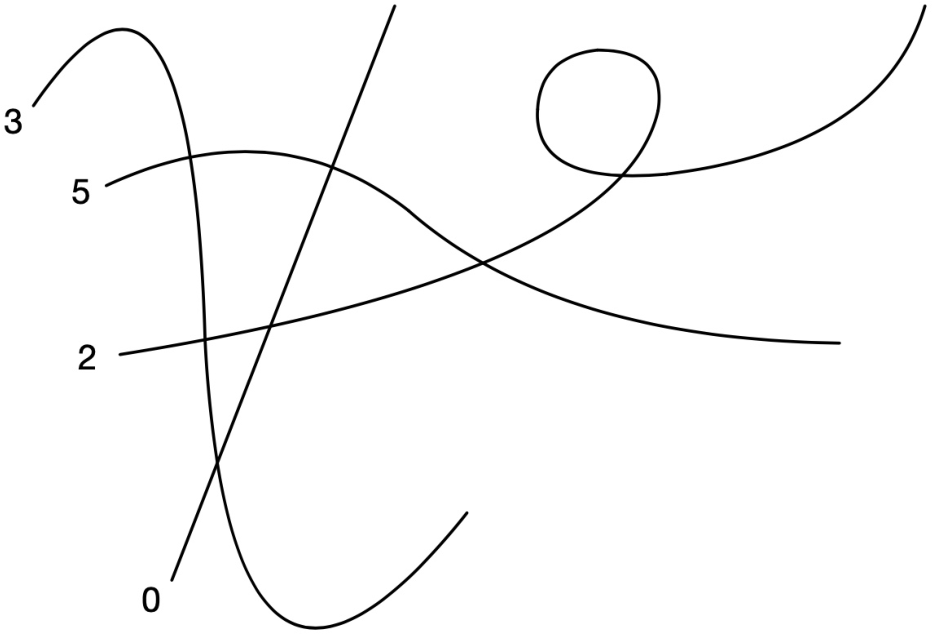
\includegraphics[width=.43\textwidth]{figures/fig-6.2.13.png}
\caption{亏格为 $14$ 的结点曲线的一个例子.}\label{src:6.2.13}
\end{figure}
\begin{remark}\label{src:6.2.14}
注意 $\delta-\nu+1$ 恰为曲线 $C$ 围出的有界连通区域数, 如图~\bookref{6.2.13} 所示. 因而可从图中方便地计算结点曲线的亏格: 将不可约分支的几何亏格相加, 再加上有界区域数. 定义~\bookref{6.3.9} 给出用对偶图作出的另一种解释. 对非结点曲线, 有类似的亏格公式, 涉及奇点的 $\delta$-不变量 (见注记~\bookref{6.2.7}).
\end{remark}
\subsection{对偶化层}\label{src:6.2.4-subsection}
由于域 $k$ 上的结点曲线 $C$ 是局部完全交, $C$ 是 Gorenstein 的, 存在对偶化线丛 $\omega_C$, 带有迹映射 $\operatorname{tr}_C:\mathrm H^1(C,\allowbreak \omega_C)\xrightarrow{\sim}k$; 见~\cite[III.7.11]{Har77} 或~\cite[\S IV]{Ser88}. 换言之, 对每个凝聚层 $F$, 自然配对
\[
\operatorname{Hom}_{\mathcal O_C}(F,\omega_C)\times\mathrm H^1(C,F)\to\mathrm H^1(C,\omega_C)\xrightarrow{\operatorname{tr}}k
\]
完美. 鉴于它对研究稳定曲线的重要性, 以下在代数闭域 $k$ 上给出 $\omega_C$ 的明确描述. 设 $\Sigma:=C^{\mathrm{sing}}$ 是奇异轨迹, $U=C\setminus\Sigma$. 设 $\pi:\widetilde C\to\allowbreak C$ 是正规化, $\widetilde\Sigma,\allowbreak \widetilde U$ 是 $\Sigma,\allowbreak U$ 的原像, 如下图:
\begin{equation}\label{src:6.2.15}
\begin{tikzcd}
\widetilde U\arrow[r,hook]\arrow[d,"\sim"']&\widetilde C\arrow[d,"\pi"]&\widetilde\Sigma\arrow[l,hook']\arrow[d]\\
\widetilde U\arrow[r,hook]&C&\Sigma.\arrow[l,hook']
\end{tikzcd}
\end{equation}
将这些点排序为 $\Sigma=\{z_1,\allowbreak \ldots,\allowbreak z_n\}$, 设 $\pi^{-1}(z_i)=\{p_i,\allowbreak q_i\}$. 由于 $\widetilde C$ 光滑, 微分层 $\Omega_{\widetilde C}$ 是对偶化线丛. 有短正合列
\begin{equation}\label{src:6.2.16}
0\to\Omega_{\widetilde C}\to\Omega_{\widetilde C}(\widetilde\Sigma)\to\mathcal O_{\widetilde\Sigma}\to0,
\end{equation}
由序列 $0\to\mathcal O_{\widetilde C}(-\widetilde\Sigma)\to\mathcal O_{\widetilde C}\to\mathcal O_{\widetilde\Sigma}\to0$ 张量 $\Omega_{\widetilde C}(\widetilde\Sigma)$ 得到. 因为 $\Omega_{\widetilde C}(\widetilde\Sigma)|_{\widetilde U}=\Omega_{\widetilde U}$, 可将 $\Omega_{\widetilde C}(\widetilde\Sigma)$ 的截面解释为 $\Omega_{\widetilde C}$ 的有理截面, 在 $\widetilde\Sigma$ 上至多有一阶极点. 在开集 $\widetilde V\subseteq\widetilde C$ 上取~\bookeqref{6.2.16} 的截面得到
\begin{equation}\label{src:6.2.17}
\begin{aligned}
0\to\Gamma(\widetilde V,\Omega_{\widetilde C})\to\Gamma(\widetilde V,\Omega_{\widetilde C}(\widetilde\Sigma))&\to\bigoplus_{y\in\widetilde V\cap\widetilde\Sigma}\kappa(y),\\
s&\mapsto(\operatorname{res}_y(s)),
\end{aligned}
\end{equation}
最后一个映射将有理截面 $s\in\Gamma(\widetilde V\cap\widetilde U,\allowbreak \Omega_{\widetilde C})$ 映到一个元组, 其在 $y\in\widetilde V\cap\widetilde\Sigma$ 处的坐标是 $s$ 在 $y$ 处的留数 $\operatorname{res}_y(s)$.
\begin{definition}[对偶化层]\label{src:6.2.18}
设 $C$ 是代数闭域 $k$ 上的结点曲线. 用~\bookeqref{6.2.15} 和~\bookeqref{6.2.17} 的记号, 定义子层 $\omega_C\subseteq\pi_*\Omega_{\widetilde C}(\widetilde\Sigma)$ 如下: 在 $V\subseteq C$ 上的截面是 $\Omega_{\widetilde C}$ 在 $\pi^{-1}(V)$ 上的有理截面 $s$, 在 $\widetilde\Sigma$ 上至多有一阶极点, 且对每个结点 $z_i\in V\cap\Sigma$ 及其原像 $p_i,\allowbreak q_i\in\pi^{-1}(V)$, 有 $\operatorname{res}_{p_i}(s)+\operatorname{res}_{q_i}(s)=0$.
\end{definition}
由定义, $\omega_C$ 位于以下两个正合列中:
\[
\begin{aligned}
0\to\omega_C\to\pi_*\Omega_{\widetilde C}(\widetilde\Sigma)&\to\bigoplus_{z_i\in\Sigma}k\to0,\\
s&\mapsto(\operatorname{res}_{p_i}(s)+\operatorname{res}_{q_i}(s)).
\end{aligned}
\]
\[
\begin{aligned}
0\to\pi_*\Omega_{\widetilde C}\to\omega_C&\to\bigoplus_{z_i\in\Sigma}k\to0,\\
s&\mapsto(\operatorname{res}_{p_i}(s)).
\end{aligned}
\]
\begin{example}[局部计算]\label{src:6.2.19}
设 $C=\Spec k[x,\allowbreak y]/(xy)$. 则 $\widetilde C=\mathbb A^1\coprod\mathbb A^1$, 分别具有坐标 $x,\allowbreak y$. $C$ 的奇异轨迹是 $\Sigma=\{0\}$, 原像 $\widetilde\Sigma$ 由两个原点组成. 此时 $\Gamma(\widetilde C,\allowbreak \Omega_{\widetilde C})=\Gamma(\mathbb A^1,\allowbreak \Omega_{\mathbb A^1})\times\Gamma(\mathbb A^1,\allowbreak \Omega_{\mathbb A^1})$, $(\frac{dx}{x},\allowbreak -\frac{dy}{y})$ 是 $\Omega_{\widetilde C}$ 的有理截面, 在 $p,\allowbreak q$ 处留数相反. 事实上, $\Gamma(C,\allowbreak \omega_C)$ 的每个截面形如
\[
\left(f(x)\frac{dx}{x},g(y)\frac{-dy}{y}\right)=\bigl(f(x)+g(y)-f(0)\bigr)\cdot\left(\frac{dx}{x},\frac{-dy}{y}\right),
\]
其中多项式 $f(x),\allowbreak g(y)$ 满足 $f(0)=g(0)$; 这正是 $(f,\allowbreak g)\in\Gamma(\widetilde C,\allowbreak \mathcal O_{\widetilde C})$ 下降为整体函数 $f(x)+g(y)-f(0)\in\Gamma(C,\allowbreak \mathcal O_C)$ 的条件. 换言之, $\omega_C\cong\mathcal O_C$, 生成元为 $(\frac{dx}{x},\allowbreak -\frac{dy}{y})$.
\end{example}
\begin{example}\label{src:6.2.20}
设 $C$ 是射影平面结点三次曲线, $\mathbb P^1\to\allowbreak C$ 是正规化, 坐标为 $[x:y]$, 使得 $0,\allowbreak \infty$ 是结点的纤维. $\mathbb P^1$ 上的有理微分 $\eta:=\frac{dx}{x}=-\frac{dy}{y}$ 满足 $\operatorname{res}_0\eta+\operatorname{res}_{\infty}\eta=0$. 不难看出 $\omega_C$ 的每个局部截面均为 $\eta$ 的倍数; 换言之, $\omega_C\cong\mathcal O_C$, 生成元为 $\eta$.
\end{example}
\begin{exercise}[细节]\label{src:6.2.21}
设 $C$ 是代数闭域 $k$ 上的连通结点射影曲线. 暂时如定义~\bookref{6.2.18} 定义子层
\[
K_C=\ker\left(\pi_*\Omega_{\widetilde C}(\widetilde\Sigma)\to\bigoplus_{z_i\in\Sigma}k\right).
\]
\begin{enumerate}[(a)]
\item 证明若 $\pi:C'\to\allowbreak C$ 是平展态射, 则 $\pi^*K_C\cong K_{C'}$.

\textit{提示:} 利用正规化与平展基变换交换.
\item 证明 $K_C$ 是线丛.

\textit{提示:} 用结点的局部结构 (\bookref{6.2.8}) 和例~\bookref{6.2.19} 中的局部计算.
\item (困难) 证明 $K_C$ 是对偶化层.

\textit{提示:} 利用正规化归结到光滑曲线的情形:
\begin{enumerate}[(i)]
\item 用 Yoneda 引理证明, 只需给出函子 $\operatorname{Pic}(C)\to\operatorname{Vect}_k$ 的同构 $\operatorname{Hom}_{\mathcal O_C}(-,\allowbreak K_C)\cong\mathrm H^1(C,\allowbreak -)^\vee$.
\item 对任意 $L\in\operatorname{Pic}(C)$, 证明将定义 $K_C$ 的正合列张量 $L^\vee$ 并取上同调, 得到等同
\[
\begin{aligned}
\operatorname{Hom}_{\mathcal O_C}(L,K_C)&\cong\mathrm H^0(C,L^\vee\otimes K_C)\\
&\cong\ker\left(\mathrm H^0(\widetilde C,\pi^*L^\vee\otimes\Omega_{\widetilde C}(\widetilde\Sigma))\to\bigoplus_{z_i\in\Sigma}k\right).
\end{aligned}
\]
\item 用短正合列 $0\to\pi_*\pi^*(L(\widetilde\Sigma))\to\allowbreak L\to\bigoplus_{z_i\in\Sigma}k\to0$, 推出
\[
\mathrm H^1(C,L)^\vee=\ker\left(\mathrm H^1(\widetilde C,\pi^*L(\widetilde\Sigma))^\vee\to\bigoplus_{z_i\in\Sigma}k\right).
\]
\item 证明 $\widetilde C$ 上的 Serre 对偶给出的同构 $\mathrm H^0(\widetilde C,\allowbreak \pi^*L^\vee\otimes\Omega_{\widetilde C}(\widetilde\Sigma))\cong\mathrm H^1(\widetilde C,\allowbreak \pi^*L(\widetilde\Sigma))^\vee$ 与到 $\bigoplus_{z_i\in\Sigma}k$ 的两个映射交换.
\end{enumerate}
另见~\cite[命题 13.2.9]{Ols16}. 其他方法见~\cite[第四章 \S 3]{Ser88}, \cite[引理 10.3.12]{Liu02} 和~\cite[第十章 \S 2]{ACG11}.
\item 若 $T\subseteq C$ 是子曲线, 补曲线为 $T^c:=\overline{C\setminus T}$, 证明
\[
\omega_C|_T=\omega_T(T\cap T^c).
\]
\end{enumerate}
\end{exercise}
\newpage
\begin{exercise}[很好的练习]\label{src:6.2.22}
设 $C$ 是代数闭域 $k$ 上的连通结点射影曲线. 设 $\pi:\widetilde C\to\allowbreak C$ 是正规化, $\widetilde\Sigma\subseteq\widetilde C$ 是结点原像的集合. 证明有等同
\[
\pi_*\mathcal H om_{\mathcal O_{\widetilde C}}(\Omega_{\widetilde C}(\widetilde\Sigma),\mathcal O_{\widetilde C})\cong\mathcal H om_{\mathcal O_C}(\Omega_C,\mathcal O_C),
\]
或等价地, $\pi_*(T_{\widetilde C}(-\widetilde\Sigma))=T_C$. 换言之, $C$ 上的正则向量场对应于 $\widetilde C$ 上在结点原像处为零的正则向量场.
\end{exercise}
\begin{remark}\label{src:6.2.23}
上述对偶化层 $\omega_C$ 的明确描述可推广到任意约化 Gorenstein 曲线 $C$. $\omega_C$ 的截面有时称为\newterm{Rosenlicht 微分}{Rosenlicht differentials}. 见~\cite[命题 6.2]{BHPV04} 和~\cite[第四章]{Ser88}.
\end{remark}
\subsection{结点曲线族}\label{src:6.2.5-subsection}
回顾, 具有一维纤维的态射 $C\to\allowbreak S$ 的相对奇异轨迹 $\operatorname{Sing}(C/S)$ 由 $\Omega_{C/S}$ 的第一个 Fitting 理想层定义; 见定义~\bookref{A.3.14}. syntomic 态射是纤维为局部完全交的 fppf 态射 (即平坦且局部有限表现); 见 \S\bookref{A.3.5-subsection}.
\begin{proposition}\label{src:6.2.24}
设 $C\to\allowbreak S$ 是概形的 fppf 态射, $s\in S$ 是点, 纤维 $C_s$ 纯一维. 点 $p\in C_s$ 是结点当且仅当 $C\to\allowbreak S$ 在 $p$ 处 syntomic, 且相对奇异轨迹 $\operatorname{Sing}(C/S)\to\allowbreak S$ 在 $p$ 处非分歧.
\end{proposition}
\begin{proof}
$C\to\allowbreak S$ 在 $p$ 处 syntomic 及 $\operatorname{Sing}(C)\to\allowbreak S$ 在 $p$ 处非分歧这两个条件, 都是关于 $s$ 上方纤维的条件. 由于 $\operatorname{Sing}(C/S)_s=\operatorname{Sing}(C_s)$, 结论由结点的刻画 (\bookref{6.2.4}) 中 (1) $\Leftrightarrow$ (4) 的等价性得到.
\end{proof}
上述刻画说明结点曲线族这一性质沿极限下降 (定义~\bookref{B.3.6}).
\begin{lemma}\label{src:6.2.25}
概形态射的以下性质沿极限下降: 每个纤维都是纯一维结点曲线的 fppf 态射.
\end{lemma}
\begin{proof}
由态射性质沿极限的下降 (\bookref{B.3.7}), 已知 fppf, syntomic, 非分歧及具有连通纯一维纤维这些性质沿极限下降. 由于相对奇异轨迹与基变换交换, 结论由命题~\bookref{6.2.24} 得到.
\end{proof}
\subsection{结点曲线族的局部结构}\label{src:6.2.6-subsection}
由光滑态射的局部结构 (\bookref{A.3.4}), 若 $C\to\allowbreak S$ 是光滑曲线族, 则 $s\in S$ 上方的每个点 $p\in C$ 平展局部地同构于相对一维仿射空间. 更准确地, 有交换图
\[
\begin{tikzcd}[column sep=small]
(C,p)\arrow[d]&(C',p')\arrow[l,"\mathrm{op}"']\arrow[r,"\text{ét}"]\arrow[d]&(S'\times_{\mathbb Z}\mathbb A^1_{\mathbb Z},(s',0))\arrow[dl]\\
(S,s)&(S',s')\arrow[l,"\mathrm{op}"']&
\end{tikzcd}
\]
其中左侧水平映射是开浸入, 右侧映射平展, 且 $S'\times_{\mathbb Z}\mathbb A^1_{\mathbb Z}=\mathbb A^1_{S'}\to\allowbreak S'$ 是 $\mathbb A^1_{\mathbb Z}\to\Spec\mathbb Z$ 的基变换. 我们为结点曲线族建立类似的局部结构, 给出结点局部结构 (\bookref{6.2.8}) 的相对版本.
\begin{theorem}[结点曲线族的局部结构]\label{src:6.2.26}
设 $\pi:C\to\allowbreak S$ 是 fppf 态射, 每个几何纤维都是曲线. 设 $p\in C$ 是点 $s\in S$ 上方纤维 $C_s$ 中的结点. 有交换图
\begin{equation}\label{src:6.2.27}
\begin{tikzcd}[column sep=small]
(C,p)\arrow[d]&(C',p')\arrow[l,"\text{ét}"']\arrow[r,"\text{ét}"]\arrow[d]&(\Spec A[x,y]/(xy-f),(s',0))\arrow[dl]\\
(S,s)&(\Spec A,s')\arrow[l,"\text{ét}"']&
\end{tikzcd}
\end{equation}
其中每个水平映射平展, $f\in A$ 是在 $s'$ 处为零的函数.
\end{theorem}
\newpage
\begin{remark}\label{src:6.2.28}
换言之, 每个结点曲线族在源与靶上平展局部地具有由函数 $f\in A$ 诱导的纤维积中的上方水平箭头的结构:
\[
\begin{tikzcd}
\Spec A[x,y]/(xy-f)\arrow[r]\arrow[d]&\Spec A\arrow[d,"f"]\\
\Spec\mathbb Z[x,y,t]/(xy-t)\arrow[r]&\Spec\mathbb Z[t].
\end{tikzcd}
\]
\end{remark}
\begin{proof}
我们给出从局部到整体的证明.

\textit{步骤 1: 归结到 $S$ 在 $\mathbb Z$ 上有限型的情形.} 用极限方法和引理~\bookref{6.2.25}.

\textit{步骤 2: 归结到 $\widehat{\mathcal O}_{C_s,\allowbreak p}\cong\kappa(s)[[x,\allowbreak y]]/(xy)$ 的情形.} 由命题~\bookref{6.2.4}, 存在有限可分域扩张 $\kappa(s)\to\allowbreak k'$ 和点 $p'\in C_s\times_{\kappa(s)}k'$, 其完备化同构于 $k'[[x,\allowbreak y]]/(xy)$. 取平展态射 $(S',\allowbreak s')\to(S,\allowbreak s)$, 使得在 $\kappa(s)$ 上有 $\kappa(s')\cong k'$, 并将 $S$ 换为 $S'$.

\textit{步骤 3: 证明对某个函数 $\widehat f\in\widehat{\mathfrak m}_s\subseteq\widehat{\mathcal O}_{S,\allowbreak s}$, 有 $\widehat{\mathcal O}_{C,\allowbreak p}\cong\widehat{\mathcal O}_{S,\allowbreak s}[[x,\allowbreak y]]/(xy-\widehat f)$.} 我们断言存在元素 $\widehat x,\allowbreak \widehat y\in\widehat{\mathcal O}_{C,\allowbreak p}$ 和 $\widehat f\in\widehat{\mathfrak m}_s\subseteq\widehat{\mathcal O}_{S,\allowbreak s}$, 满足 $\widehat x\widehat y-\widehat f=0$. 为此, 归纳构造 $n\geq0$ 时的元素 $x_n,\allowbreak y_n\in\widehat{\mathcal O}_{C,\allowbreak p}$ 和 $f_n\in\widehat{\mathfrak m}_s$, 它们相容 (即 $x_{n+1}\equiv x_n\pmod{\mathfrak m^{n+1}}$ 等), 且
\begin{equation}\label{src:6.2.29}
x_ny_n-f_n\in\widehat{\mathfrak m}_s^{n+1}\widehat{\mathcal O}_{C,p}.
\end{equation}
定义 $\widehat x=\lim_n x_n$, $\widehat y=\lim_n y_n$, $\widehat f=\lim_n f_n$, 即得断言.

初始情形 $n=0$ 由步骤 2 处理: 设 $\overline x,\allowbreak \overline y\in\widehat{\mathcal O}_{C_s,\allowbreak p}$ 是 $x,\allowbreak y$ 在同构 $\widehat{\mathcal O}_{C_s,\allowbreak p}\cong\kappa(s)[[x,\allowbreak y]]/(xy)$ 下的像, 取 $x_0,\allowbreak y_0\in\widehat{\mathcal O}_{C,\allowbreak p}$ 为它们在满射 $\widehat{\mathcal O}_{C,\allowbreak p}\to\widehat{\mathcal O}_{C_s,\allowbreak p}$ 下的任意提升, 并令 $f_0=0$. 假设已构造满足~\bookeqref{6.2.29} 的 $x_n,\allowbreak y_n,\allowbreak f_n$, 写成
\[
x_ny_n-f_n=\sum_i a_i b_i,\qquad a_i\in\widehat{\mathfrak m}_s^{n+1},\quad b_i\in\widehat{\mathcal O}_{C,p}.
\]
由于 $x_n,\allowbreak y_n$ 生成 $p$ 在纤维 $C_s$ 中的极大理想, 可利用剩余域上的等式 $\kappa(s)=\kappa(p)$, 找到 $a'_i\in\widehat{\mathcal O}_{S,\allowbreak s}$ 和 $b'_i,\allowbreak b''_i\in\widehat{\mathcal O}_{C,\allowbreak p}$, 使得
\[
b_i-(x_nb'_i+y_nb''_i+a'_i)\in\widehat{\mathfrak m}_s\widehat{\mathcal O}_{C,p}.
\]
然后定义
\[
x_{n+1}=x_n-\sum_i a_i b''_i,\quad y_{n+1}=y_n-\sum_i a_i b'_i,\quad f_{n+1}=f_n+\sum_i a_i a'_i,
\]
并验证
\[
\begin{aligned}
x_{n+1}y_{n+1}-f_{n+1}
&=(x_n-\sum_i a_i b''_i)(y_n-\sum_i a_i b'_i)-(f_n+\sum_i a_i a'_i)\\
&=(x_ny_n-f_n)-x_n\sum_i a_i b'_i-y_n\sum_i a_i b''_i-\sum_i a_i a'_i+\sum_{i,j}a_i a_j b''_i b'_j\\
&=\sum_i a_i b_i-x_n\sum_i a_i b'_i-y_n\sum_i a_i b''_i-\sum_i a_i a'_i+\sum_{i,j}a_i a_j b''_i b'_j\\
&=\sum_i\underbrace{a_i}_{\widehat{\mathfrak m}_s^{n+1}}\underbrace{(b_i-x_nb'_i-y_nb''_i-a'_i)}_{\widehat{\mathfrak m}_s\widehat{\mathcal O}_{C,p}}+\sum_{i,j}\underbrace{a_i a_j}_{\widehat{\mathfrak m}_s^{2(n+1)}}b''_i b'_j
\end{aligned}
\]
属于 $\widehat{\mathfrak m}_s^{n+2}\widehat{\mathcal O}_{C,\allowbreak p}$.

建立断言后, 有良定义的 $\mathcal O_{S,\allowbreak s}$-代数同态
\[
\widehat{\mathcal O}_{S,s}[[x,y]]/(xy-\widehat f)\to\widehat{\mathcal O}_{C,p},
\]
由 $x\mapsto\widehat x$, $y\mapsto\widehat y$ 定义. 模 $\widehat{\mathfrak m}_s$ 后它满射, 所以由完备 Nakayama 引理 (\bookref{B.5.6}(2)) 满射; 由平坦性局部判据的一个版本 (引理~\bookref{A.2.8}) 单射, 因而是同构.

\textit{步骤 4 (从形式邻域到平展邻域): 将步骤 3 中形式邻域的同构延伸到平展邻域.} 由步骤 3, 有图
\[
\begin{tikzcd}[column sep=small]
C\times_S\Spec\widehat{\mathcal O}_{S,s}\arrow[dr]&&\Spec\widehat{\mathcal O}_{S,s}[x,y]/(xy-\widehat f)\arrow[dl]\\
&\Spec\widehat{\mathcal O}_{S,s}&
\end{tikzcd}
\]
其中点 $(p,\allowbreak s)\in C\times_S\Spec\widehat{\mathcal O}_{S,\allowbreak s}$ 和 $(s,\allowbreak 0)\in\Spec\widehat{\mathcal O}_{S,\allowbreak s}[x,\allowbreak y]/(xy-\widehat f)$ 的完备化同构. Artin 逼近 (\bookref{B.5.21}) 的一个推论说明存在定义在 $\Spec\widehat{\mathcal O}_{S,\allowbreak s}$ 上的平展态射
\begin{equation}\label{src:6.2.30}
\begin{tikzcd}[column sep=small]
&(U,u)\arrow[dl]\arrow[dr]&\\
(C\times_S\Spec\widehat{\mathcal O}_{S,s},(p,s))&&(\Spec\widehat{\mathcal O}_{S,s}[x,y]/(xy-\widehat f),(s,0)).
\end{tikzcd}
\end{equation}
将 $S$ 换为 $s$ 的仿射开邻域后, 可假设 $S=\Spec A$ 仿射. 由 Néron--Popescu (\bookref{B.5.15}), 可将 $\widehat{\mathcal O}_{S,\allowbreak s}=\operatorname{colim}B_\lambda$ 写成光滑 $A$-代数的有向余极限. 置 $S_\lambda=\Spec B_\lambda$, $C_\lambda=C\times_S S_\lambda$, $U_\lambda=U\times_S S_\lambda$. 对 $\lambda\gg0$, $\widehat f\in\widehat{\mathcal O}_{S,\allowbreak s}$ 是某个元素 $f_\lambda\in B_\lambda$ 的像, $x,\allowbreak y$ 在 $\Gamma(U,\allowbreak \mathcal O_U)$ 中的拉回是 $\Gamma(U_\lambda,\allowbreak \mathcal O_{U_\lambda})$ 中元素在 $U\to\allowbreak U_\lambda$ 下的拉回. 这给出 $S_\lambda$ 上的交换图
\[
\begin{tikzcd}[column sep=small]
&U_\lambda\arrow[dl]\arrow[dr]&\\
C_\lambda&&\Spec B_\lambda[x,y]/(xy-f_\lambda),
\end{tikzcd}
\]
沿 $\Spec\widehat{\mathcal O}_{S,\allowbreak s}\to\allowbreak S_\lambda$ 基变换后成为~\bookeqref{6.2.30}. 由态射性质沿极限的下降 (\bookref{B.3.7}), 平展性沿极限下降, 所以对 $\lambda\gg0$, 映射 $U_\lambda\to\allowbreak C_\lambda$ 和 $U_\lambda\to\Spec B_\lambda[x,\allowbreak y]/(xy-f_\lambda)$ 平展. 令 $u_\lambda=(u,\allowbreak s_\lambda)\in U_\lambda$, 得到交换图
\[
\begin{tikzcd}[column sep=small]
(C,p)\arrow[d]&(U_\lambda,u_\lambda)\arrow[l,"\mathrm{sm}"']\arrow[r,"\text{ét}"]\arrow[d]&(\Spec B_\lambda[x,y]/(xy-f_\lambda),(s_\lambda,0))\arrow[dl]\\
(S,s)&(\Spec B_\lambda,s_\lambda)\arrow[l,"\mathrm{sm}"']&
\end{tikzcd}
\]
这就是所需的图~\bookeqref{6.2.27}, 但左侧水平箭头光滑而非平展. 由于光滑映射平展局部地有截面 (推论~\bookref{A.3.5}), 存在平展映射 $(\Spec A,\allowbreak s')\to(S,\allowbreak s)$ 和 $S$ 上的映射 $(\Spec A,\allowbreak s')\to(S_\lambda,\allowbreak s_\lambda)$. 令 $C':=U_\lambda\times_{S_\lambda}\Spec A$, $p'=(u_\lambda,\allowbreak s')$, 即得结论. 另见~\cite[Tag 0CBY]{SP}.
\end{proof}
\begin{exercise}\label{src:6.2.31}
按以下方式给出避免 Artin 逼近和 Néron--Popescu 的另一证明:
\begin{enumerate}[(i)]
\item 归结到 $S$ 在 $\mathbb Z$ 上有限型的情形.
\item 归结到 $C\to\allowbreak S$ 是仿射概形的 syntomic 态射的情形, 其几何纤维连通且至多有两个不可约分支, $\operatorname{Sing}(C/S)\to\allowbreak S$ 是同构或由非零因子定义的闭浸入.
\item 利用正规化和 Hensel 化的性质, 处理 $\operatorname{Sing}(C/S)=S$ 与 $\operatorname{Sing}(C/S)=V(f)$ 两种情形.
\end{enumerate}
\end{exercise}
